%%%%%%%%%%%%%%%%%%%%%%%%%%%%%%%%%%%%%%%%%%%%%%%%%%%%%%%%%%%%%%%%%%%%%%
%%                     And
%%%%%%%%%%%%%%%%%%%%%%%%%%%%%%%%%%%%%%%%%%%%%%%%%%%%%%%%%%%%%%%%%%%%%%
\subsection{Glyph: \glyph{And}}\label{sec:and}

The glyph \glyph{and} is used to denote that all the \glyph{EPNs} linked as input are necessary to produce the output. For instance a modulator A \glyph{and} a modulator B, when both present modulate the flux of a process. \glyph{And} is represented by a circle carrying the word ``AND''.

\begin{figure}[H]
  \centering
  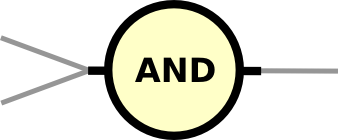
\includegraphics[scale = 0.5]{images/and}
  \caption{The \PD glyph for \glyph{and}. Only two inputs are represented, but more would be allowed.}
  \label{fig:and}
\end{figure}
